\documentclass[10pt]{article}
\usepackage{amsmath,textcomp,amssymb,geometry,graphicx,enumerate,tikz,algorithm,algpseudocode,pifont}
\usetikzlibrary{calc}
\usetikzlibrary{datavisualization}
\usetikzlibrary{datavisualization.formats.functions}


\textheight=9in
\textwidth=7in
\topmargin=-.75in
\oddsidemargin=-0.25in
\evensidemargin=-0.25in

\usepackage{listings}
\lstnewenvironment{codeblock}
    {\lstset{language=Python,
      showspaces=false,
      showtabs=false,
      breaklines=true,
      mathescape=true,
      showstringspaces=false,
      breakatwhitespace=true,
      commentstyle=\textit,
      keywordstyle=\textbf,
      basicstyle=\ttfamily,
      escapechar=`,
      moredelim={**[is][{\color{RoyalBlue}}]{\^^M\\beginsol}{\^^M\\endsol}},
      moredelim={[is][{\color{RoyalBlue}}]{\^^M\\beginexp}{\^^M\\endexp}},
    }}
    {}

\begin{document}
\section*{03/09/2016}
	\subsection*{Kernels} continued
	\begin{itemize}
		\item \underline{Kernel Perceptrons}
		\item Note: Everywhere below, we can replace $X_{i}$ with $\phi(X_{i})$
		\end{itemize}

\begin{codeblock}
	Perceptron Algorithm:
	    while (some $y_{i}X_{i} \cdot w < 0$):
	        $w \leftarrow w + \epsilon y_{i}x_{i}$
	    while (still have test points $z$):
	        $f(z) \leftarrow w^{T}x$
\end{codeblock}
		\begin{itemize}
		\item Kernelize with $w=X^{T}a$; $X_{i}\cdot w = (XX^{T}a)_{i} = (Ka)_{i}$.
		\end{itemize}

\begin{codeblock}
	Dual Perceptron Algorithm:
	    $a = [y_{1}, 0, \dots, 0]^{T}$
	    $K_{ij} = K(X_{i}, X_{j}) \ \forall i,j$
	    while (some $y_{i}(Ka)_{i} \cdot w < 0$):
	        $a \leftarrow a + \epsilon y_{i}$
	    while (still have test points $z$):
	        $f(z) \leftarrow \sum_{j=1}^{n} a_{j}K(X_{j},z)$
\end{codeblock}
		\begin{itemize}
		\item Computing $K_{ij} \Leftarrow \mathcal{O}(n^{2}d)$ time (kernel trick).
		\item Optimization for first while loop: maintain $Ka$, $\mathcal{O}(n)$ time.
		\item Second loop runs in $\mathcal{O}(nd)$ time or we can compute $w=X^{T}a$ once in $\mathcal{O}(nd')$ time and evaluate test points in $\mathcal{O}(d')$ time per point, where $d'$ is the length of $\phi(\cdot)$.
	\end{itemize}

	\subsection*{Kernel Logistic Regression}
	\
	\begin{itemize}
		\item Stochastic gradient ascent step:
			\begin{align*}
				a_{i} \leftarrow a_{i} + \epsilon(y_{i} - s((Ka)_{i}))\\
			\end{align*}
		\item Gradient ascent step:
			\begin{align*}
				a \leftarrow a + \epsilon(y_{i} - s((Ka)) \Leftarrow \text{ applying s component-wise to vector } Ka \\
			\end{align*}	
		\item for each test point $z$: $h(z) \leftarrow s(\sum_{j=1}^{n} a_{j}k(X_{j}, z))$.
	\end{itemize}
	
	\subsection*{The Gaussian Kernel}
	\
	\begin{itemize}
		\item \underline{Gaussian kernel}, aka \underline{radial basis function kernel}
		\item There exists a $\phi(x)$ such that:
			\begin{align*}
				k(x, z) = e^{(-\frac{|x-z|^{2}}{2\sigma^{2}})}
			\end{align*}
		\item Key observation: $h(z) = s(\sum_{j=1}^{n} a_{j}k(X_{j}, z))$ is a linear combination of Gaussian centered at samples.
		\item Very popular in practice:
			\begin{itemize}
				\item Gives very smooth $h$
				\item Behaves somewhat like k-nearest neighbor, but smoother.
				\item Oscillates less than polynomial (depending on $\sigma$).
				\item $k(x,z)$ can be interpreted as a "similarity measure" $y$ value more influenced by points around it.
				\item Gaussian is maximum when $x=z$, goes to 0 as distance increases.
				\item Samples "vote" for value at $z$, but closer samples get bigger vote.
			\end{itemize}
		\item $\sigma$ trades off bias vs. variance:
			\begin{itemize}
				\item larger $\sigma \rightarrow$ wider Gaussians, smoother $h \rightarrow$ more bias, less variance.
				\item Choose by (cross)-validation.
			\end{itemize}
	\end{itemize}
	
	\subsection*{Subset Selection}
	\begin{itemize}
		\item All features increase variance, but not all features reduce bias.
		\item Idea: Identify poorly predictive features, ignore them (weight zero). Less over-fitting, lower test errors.
		\item 2nd motivation: Inference. Simpler models convey interpretable wisdom. Useful in all classification and regression methods. Sometimes it's hard: Different feature can partly encode some info. Combinatorially hard to choose best feature subset.
		\item Algorithm: Best subset selection. Try all $2^{d} - 1$ nonempty subsets of features. Choose the best model by cross-validation. This is very slow!
		\item Heuristic: \underline{Forward stepwise selection}.
		\begin{itemize}
			\item Start with \underline{null model} (0 features); repeatedly add best feature. Repeat until test errors start increasing (due to over-fitting).
			\item Requires training $\mathcal{O}(d^{2})$ models instead of $\mathcal{O}(2^{d})$.
			\item Not perfect.
		\end{itemize}
		\item Heuristic: \underline{Backward stepwise selection}.
		\begin{itemize}
			\item Start with all $d$ features; repeatedly remove feature whose removal gives best reduction in test error.
			\item Also trains $\mathcal{O}(d^{2})$ models.
		\end{itemize}
		\item If you think there's only a few good features do forward, if you think most features will be good do backwards.
	\end{itemize}
	
	\subsection*{Lasso (Tibsharani, 1996)}
	\begin{itemize}
		\item Regression with regularization: (1) + (A) + $\ell_{1}$ penalized mean loss (e) "Least absolute shrinkage and selection operator"
		\item Optimization problem:
		\begin{center}
			\begin{tabular}{|c|}
				\hline
				Find $w$ that minimizes $|Xw-y|^{2} + \lambda|w'|_{1}$\\
				\hline
			\end{tabular}\\
		\end{center}
		where $|w'|_{1} = \sum_{i=1}^{n}|w_{i}|$.
		\item Recall ridge regression: isosurfaces of $|w'|_{2}^{2}$ are hyperspheres. 
		\item The isosurfaces of $|w'|_{1}$ are \underline{cross-polytopes}.
		\item The unit cross-polytope is the convex hull of all the positive and negative unit coordinate vectors.
		\begin{center}
			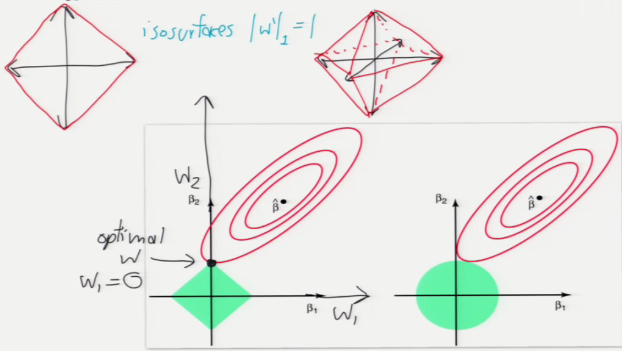
\includegraphics[scale=0.6]{../images/lassol1}
			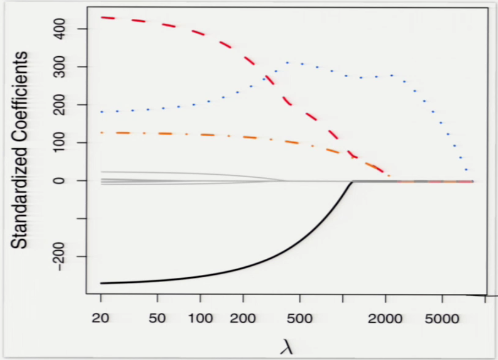
\includegraphics[scale=0.6]{../images/standarizesweights}
		\end{center}
		
		\item Algorithms to optimize: subgradient descent, least-angle regression (LARS), forward stagewise.
	\end{itemize}	
\end{document}
